\documentclass[xcolor=dvipsnames]{beamer}
\usepackage{lmodern}
\usepackage[T1]{fontenc}
\usepackage[english]{babel}
\usepackage[utf8]{inputenc}

\usepackage{manfnt}
\usepackage{wasysym}
\usepackage{listings}
\usepackage{graphicx}
\usepackage{url}
\usepackage{ulem}
\usepackage{marvosym}
\usepackage{proof}
\usepackage{array}
\setbeamertemplate{navigation symbols}{}

\title[Demystifying Debugging]{{\bf Demystifying Debugging}}
\subtitle[]{{\em when getting it right the first time every time fails}}
\author[Ben Blum]{Ben Blum \texttt{(bblum@andrew.cmu.edu)}}

\institute[98-172]{Great Practical Ideas for Computer Scientists}
\date[]{2012, November 8}

\setbeamertemplate{footline}{\hspace*{.5cm}\scriptsize{\insertauthor\hspace*{50pt} \hfill\insertframenumber\hspace*{.5cm}}}

\usecolortheme{seahorse}
\usecolortheme{rose}
\useoutertheme{infolines}

\usecolortheme[named=RoyalBlue]{structure}

\newcommand\noob{\mathsf{noob}}
\newcommand\gibs{\mathsf{gibs}}
\newcommand\dps{\mathsf{dps}}
\newcommand\squig\rightsquigarrow
\newcommand\Coloneqq{\mathrel{\mathop{::}}=}
\newcommand\dmg{\text{\Laserbeam}}
\newcommand\delter\delta
\newcommand\alpher\alpha
\newcommand\defnor{\text{ }|\text{ }}

\newcommand\pimp{\mathop{\supset}}
\newcommand\pand{\mathop{\wedge}}
\newcommand\por{\mathop{\vee}}
\newcommand\ptrue{\top}
\newcommand\pfalse{\bot}


\begin{document}
% \renewcommand{\inserttotalframenumber}{28} % If you want to hide bonus slides
\normalem
\begin{frame}
	\titlepage
\end{frame}

%%%%%%%%%%%%%%%%%%%%%%%%%%%%%%%%%%%%%%%%%%%%%%%%%%%%%%%%%%%%%%%%%%%%%%%%%%%%%%%%
%%%%%%%%%%%%%%%%%%%%%%%%%%%%%%%%%%%%%%%%%%%%%%%%%%%%%%%%%%%%%%%%%%%%%%%%%%%%%%%%
%%%%%%%%%%%%%%%%%%%%%%%%%%%%%%%%%%%%%%%%%%%%%%%%%%%%%%%%%%%%%%%%%%%%%%%%%%%%%%%%

\newcommand\linegap{\vspace{0.2in}}
\newcommand\breakslide[1]{\begin{frame}{} \begin{center} \Large #1 \end{center} \end{frame}}
\newcommand\related[1]{\textsuperscript{\em [#1]}}
\newcommand\hilight[2]{\color{#1}#2\color{black}}
\definecolor{grey}{RGB}{127,127,127}
\definecolor{darkcyan}{RGB}{0,127,127}
\definecolor{olivegreen}{RGB}{0,127,0}
\definecolor{violet}{RGB}{127,0,127}
\definecolor{brickred}{RGB}{127,0,0}
\definecolor{brown}{RGB}{127,63,0}


\begin{frame}{Outline}
	\begin{columns}[l]
	\column{0.05\textwidth}
	\column{0.5\textwidth}
	\textbf{Why teach debugging?}
		% brief motivation
		% toolbox
	\linegap

	\textbf{``Tell Me a Story''}
	\begin{itemize}
		\item The good debugger's attitude
			% "get more operators"
	\end{itemize}
	\linegap

	{\bf Two Main Approaches}
	\begin{itemize}
		\item Time Travel
			% small test cases / minimize the test case
		\item Space Travel
			% printf debugging
			% invariant checkers and asserts
	\end{itemize}
	\linegap

	{\bf Assorted Tricks}
	\begin{itemize}
		\item Question assumptions
		\item Draw pictures
		\item Binary search
	\end{itemize}
	\column{0.45\textwidth}
	%\begin{center}
	%	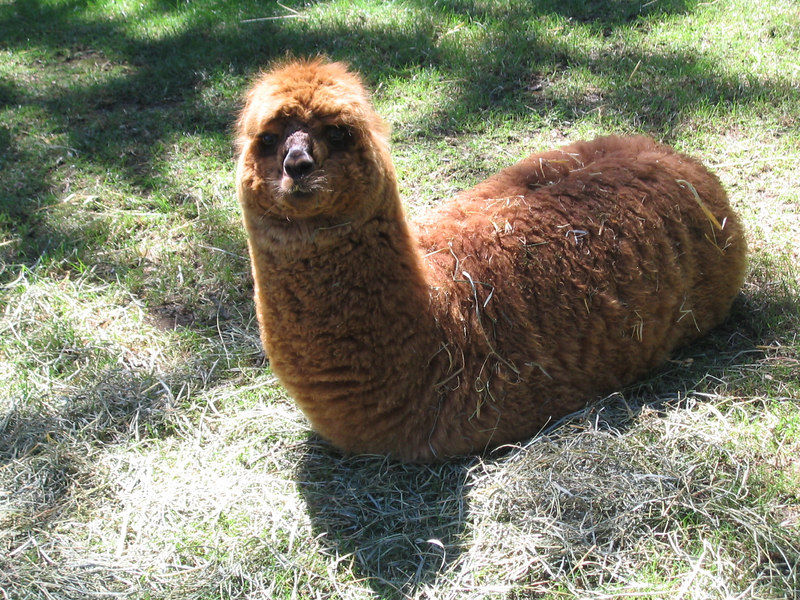
\includegraphics[width=0.9\textwidth]{vip1066720.jpg}
	%\end{center}
	\end{columns}
\end{frame}

%%%%%%%%%%%%%%%%%%%%%%%%%%%%%%%%%%%%%%%%%%%%%%%%%%%%%%%%%%%%%%%%%%%%%%%%%%%%%%%%
\section{Motivation}
%%%%%%%%%%%%%%%%%%%%%%%%%%%%%%%%%%%%%%%%%%%%%%%%%%%%%%%%%%%%%%%%%%%%%%%%%%%%%%%%

\begin{frame}{``The Universal Backup Plan''}
	\textbf{15-112, 15-122, 15-150, ...}
	\begin{itemize}
		\item What do these classes all have in common?
		\pause
		\item How to write code that {\em works}
	\end{itemize}
	\pause
	\linegap

	{\bf 98-172}
	\begin{itemize}
		\item What to do with code that {\em doesn't}
	\end{itemize}
	% TODO: a picture goes here -- blank slate vs equipped/prepared technician
\end{frame}

\begin{frame}{Take-away}
	This lecture's goal: To give you a {\em framework} for thinking when faced with buggy code.
	\linegap

	\textbf{Debugging toolbox}
	\begin{itemize}
		\item Two major {\em strategies} for approaching bugs
		\item Assorted {\em tactics} for applying to broken programs
	\end{itemize}
	% Say: "It's not, e.g., a checklist of bugs that you can just run down and test one-by-one; it's more abstract than that. You have to use your brain to figure out how to apply each tool. But the hope is that you won't feel lost staring at a blank slate of possible approaches.
\end{frame}


%%%%%%%%%%%%%%%%%%%%%%%%%%%%%%%%%%%%%%%%%%%%%%%%%%%%%%%%%%%%%%%%%%%%%%%%%%%%%%%%
\section{Storytelling}
%%%%%%%%%%%%%%%%%%%%%%%%%%%%%%%%%%%%%%%%%%%%%%%%%%%%%%%%%%%%%%%%%%%%%%%%%%%%%%%%

\begin{frame}{The Essence of Debugging}
	...is {\bf telling a good story.}
	\pause
	\linegap

	Two stories, actually:
	\begin{itemize}
		\item What you wanted to happen
		\item What the computer actually did
	\end{itemize}
	\pause
	Your bug: The point where the stories diverge
	\begin{itemize}
		\item Can you describe that point in as much detail as possible?
	\end{itemize}
\end{frame}

\begin{frame}{The Essence of Debugging}
	Because you will write unique bugs, you will be telling a story nobody else knows.

	\linegap
	``Plot summaries'' are often not enough: My program crashes...
	\pause
	\begin{itemize}
		\item with a segmentation fault...
		\pause
		\begin{itemize}
			\item in \texttt{take\_final\_exam()}...
			\pause
			\begin{itemize}
				\item because \texttt{study\_for\_final()} passed \texttt{NULL} to it.
				\item There we go!
			\end{itemize}
		\end{itemize}
	\end{itemize}
\end{frame}

\begin{frame}{Aside: Asking for Help}
	This DOESN'T mean...
	\begin{itemize}
		\item That TAs can't help you without a detailed story
		\item (That you shouldn't seek help until you've already found your bug?!)
	\end{itemize}
	\pause
	\linegap

	This does mean...
	\begin{itemize}
		\item You need a detailed story to understand your bug.
		\item If the TA doesn't know the story, how can they help?
		\pause
		\begin{itemize}
			\item They know what you should do to make your story better.
		\end{itemize}
	\end{itemize}
\end{frame}

\begin{frame}{Running Example}
	\textbf{Broken \texttt{insert\_sorted}}

	\linegap
	Sorts OK into the middle and front of list:
	\begin{itemize}
		\item \texttt{insert\_sorted} $\quad \hilight{olivegreen}{10} \quad  [20,30] \quad \Rightarrow \quad [\hilight{olivegreen}{10},20,30]$
		\item \texttt{insert\_sorted} $\quad \hilight{olivegreen}{32} \quad  [16,64] \quad \Rightarrow \quad [16,\hilight{olivegreen}{32},64]$
	\end{itemize}

	\linegap
	But not so great at the end:
	\begin{itemize}
	\item \texttt{insert\_sorted} $\quad \hilight{red}{100}  \quad [97,98,99] \quad \Rightarrow \quad [97,98,\hilight{red}{100},99]$
	\end{itemize}
\end{frame}

\begin{frame}{Running Example}
	\textbf{Broken \texttt{insert\_sorted}}

	\linegap
	In case you're curious, here's the bug:

	\linegap
		\texttt{~~~~insert\_sorted(list,~element)~\{} \\
			\texttt{~~~~~~~~\hilight{olivegreen}{int}~i~=~\hilight{brickred}{0};} \\
		\texttt{~~~~~~~~\hilight{brown}{while}~(i~<~length(list))~\{~\hilight{darkcyan}{//~Should~be~"<="!}} \\
		\texttt{~~~~~~~~~~~~\hilight{brown}{if}~(element~<~list[i])~\{} \\
		\texttt{~~~~~~~~~~~~~~~~\hilight{brown}{break};} \\
		\texttt{~~~~~~~~~~~~\}} \\
		\texttt{~~~~~~~~\}} \\
		\texttt{~~~~~~~~insert\_at\_index(list,~element,~i);} \\
		\texttt{~~~~\}} \\
\end{frame}

\begin{frame}{Running Example}
	\textbf{Broken \texttt{insert\_sorted}}

	\linegap
	Consider this test case:

	\linegap
		\texttt{~~~~input~=~\hilight{brickred}{[99,~42,~3,~100,~87,~56,~22,~38]};} \\
		\texttt{~~~~output~=~\hilight{brickred}{[]};} \\
		\texttt{~~~~\hilight{brown}{foreach}~element~\hilight{brown}{in}~input~\{} \\
		\texttt{~~~~~~~~insert\_sorted(output,~element);} \\
		\texttt{~~~~\}} \\
		\texttt{~~~~\hilight{brown}{return}~is\_sorted(output);~\hilight{darkcyan}{//~returns~false~:(}} \\
	\linegap

	\pause
	\begin{itemize}
		\item Says there is a bug
		\item Doesn't say where
	\end{itemize}
	\pause
	{\bf How can we improve it?}
\end{frame}

%%%%%%%%%%%%%%%%%%%%%%%%%%%%%%%%%%%%%%%%%%%%%%%%%%%%%%%%%%%%%%%%%%%%%%%%%%%%%%%%
\section{Strategies}
%%%%%%%%%%%%%%%%%%%%%%%%%%%%%%%%%%%%%%%%%%%%%%%%%%%%%%%%%%%%%%%%%%%%%%%%%%%%%%%%

\subsection{Time Travel}

\breakslide{``Time Travel'': {\bf When} things go wrong\dots}

\begin{frame}{Telling a Story of Time}
	Remember, two stories: Expected outcome vs Actual outcome

	\linegap
	{\em Time-wise}, this means ``It did X, then should have done Y but did Z''
	\begin{itemize}
		\item Are X,Y,Z in enough detail?
		\item Did something important happen in between?
	\end{itemize}
\end{frame}

\begin{frame}{Telling a Story of Time}
	Our test case tells this story:

	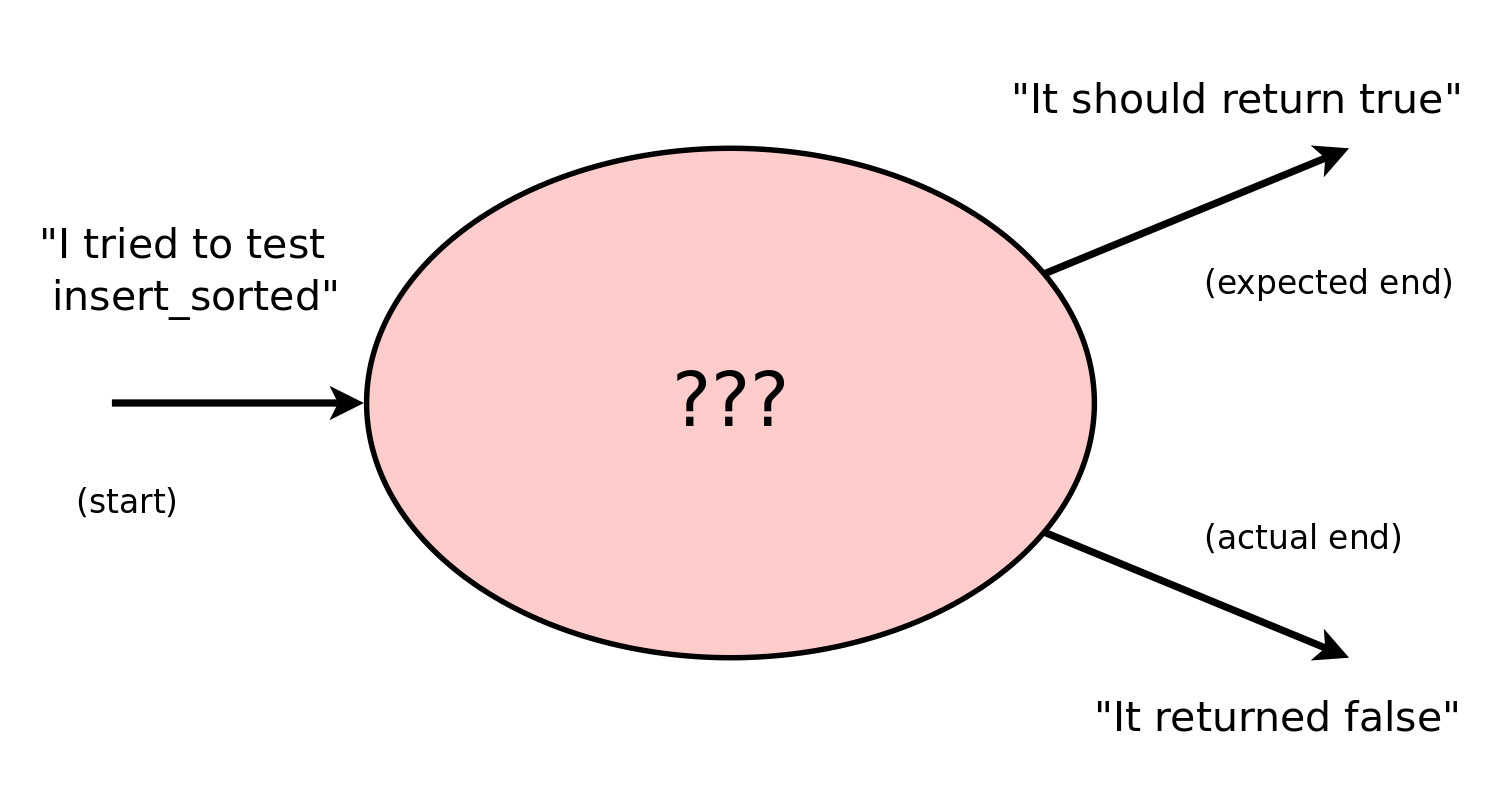
\includegraphics[width=\textwidth]{time0.png}
\end{frame}

\begin{frame}{Print Debugging}
	Make your program print its state during the big pink ``???''.
	\begin{itemize}
		\item Reduce how much of the story the ``???'' obscures.
		\begin{itemize}
			\item Find the {\em last} print {\em before} the bug
			\item Find the {\em first} print {\em after} the bug
		\end{itemize}
	\end{itemize}
	\pause

	\linegap
		\texttt{~~~~\hilight{brown}{foreach}~element~\hilight{brown}{in}~input~\{} \\
		\texttt{~~~~~~~~\hilight{olivegreen}{print(output);}} \\
		\texttt{~~~~~~~~insert\_sorted(output,~element);} \\
		\texttt{~~~~\}} \\

\end{frame}

\begin{frame}{Print Debugging}
	Old story:

	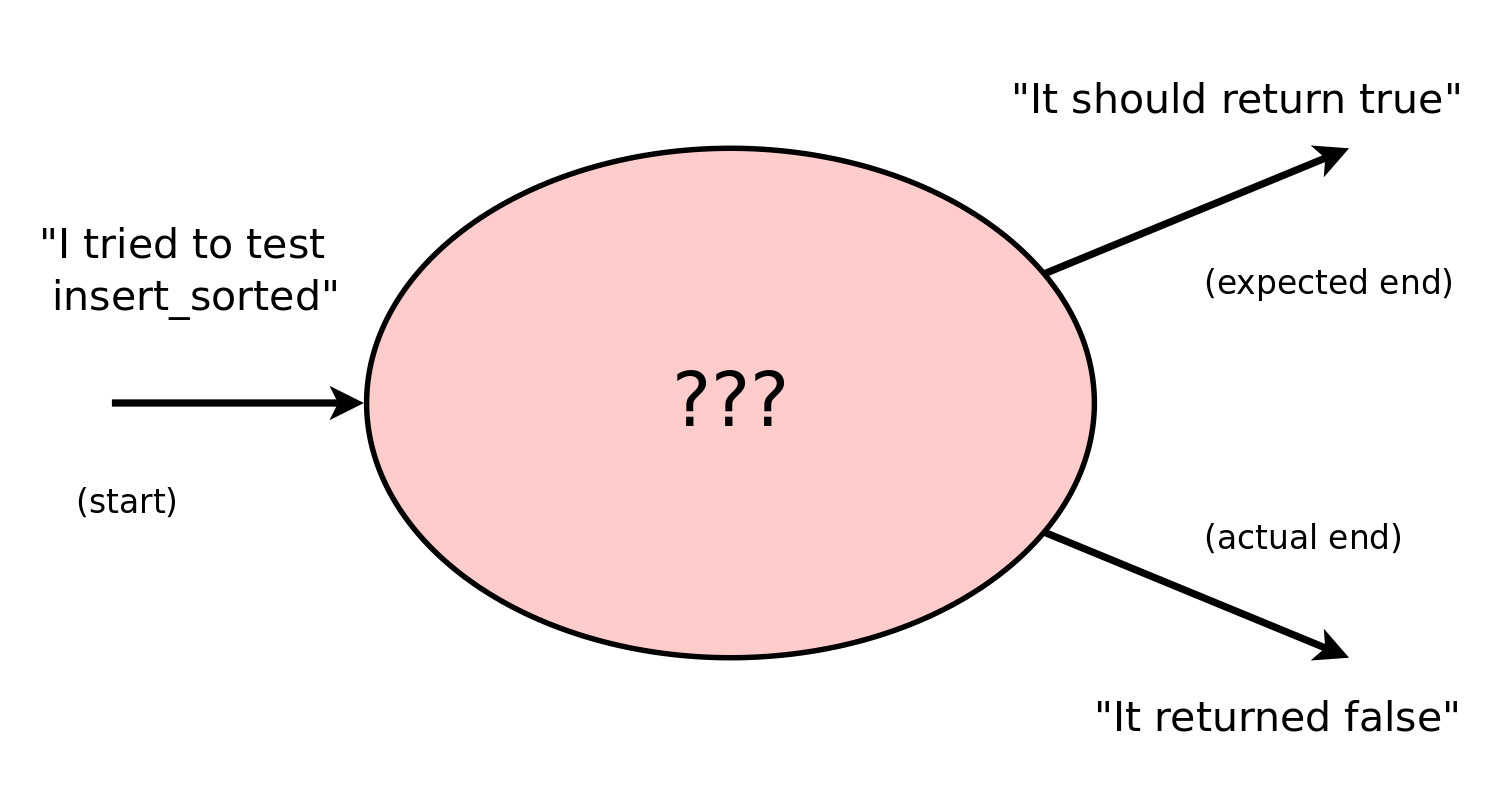
\includegraphics[width=\textwidth]{time0.png}
\end{frame}
\begin{frame}{Print Debugging}
	New story:

	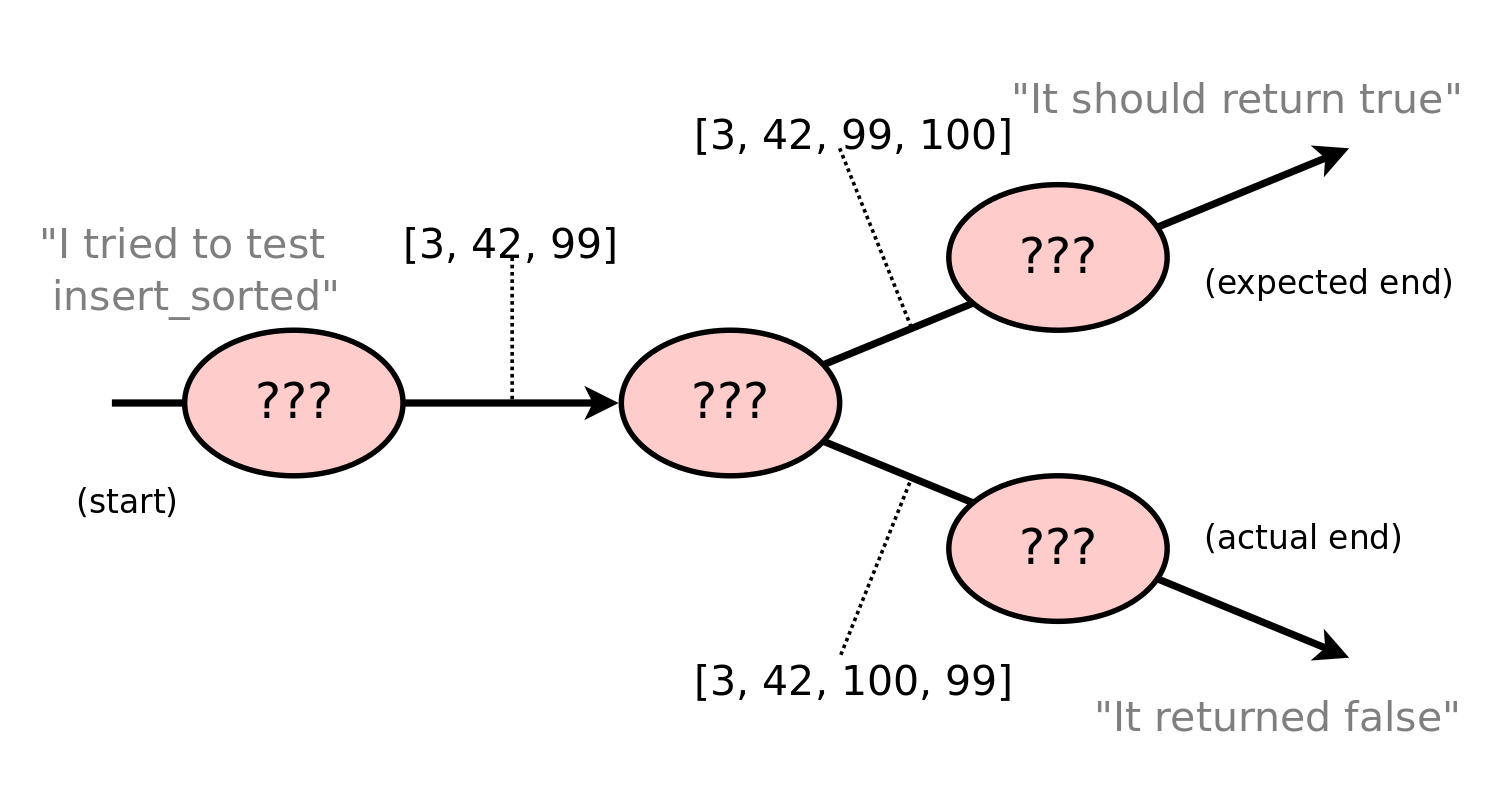
\includegraphics[width=\textwidth]{time1.png}
\end{frame}

\begin{frame}{Asserts: Stealthier, more concealable prints}
	Adding print statements everywhere is very verbose
	\begin{itemize}
		\item Pro: Get to see everything
		\item Con: Have to look at everything
	\end{itemize}
	\pause
	15-122's C0 ``contracts'' are assertions
	\begin{itemize}
		\item You don't need to use C0 to write assert-ful code
		\item Asserts can go anywhere, not just around functions/loops
	\end{itemize}
	\pause
	\linegap

	\texttt{~~~~\hilight{brown}{if}~(something\_that\_should\_never\_happen)~\{} \\
	\texttt{~~~~~~~~print(\hilight{brickred}{"oh~no,~it~happened!"});} \\
	\texttt{~~~~~~~~crash();} \\
	\texttt{~~~~\}} \\
\end{frame}
\begin{frame}{Asserts: Stealthier, more concealable prints}
	Adding print statements everywhere is very verbose
	\begin{itemize}
		\item Pro: Get to see everything
		\item Con: Have to look at everything
	\end{itemize}
	15-122's C0 ``contracts'' are assertions
	\begin{itemize}
		\item You don't need to use C0 to write assert-ful code
		\item Asserts can go anywhere, not just around functions/loops
	\end{itemize}
	\linegap

		\texttt{~~~~\hilight{brown}{foreach}~element~\hilight{brown}{in}~input~\{} \\
		\texttt{~~~~~~~~insert\_sorted(output,~element);} \\
		\texttt{~~~~~~~~\hilight{olivegreen}{assert(is\_sorted(output));}} \\
		\texttt{~~~~\}} \\
\end{frame}

\begin{frame}{Aside: 15-213 ``malloc lab''}
	At the end of 15-213, you will implement \texttt{malloc()}.
	\begin{itemize}
		\item Complex, low-level systems code
		\item Very easy to end up with difficult, subtle bugs
		\begin{itemize}
			\item Your data winds up in the wrong place, gets clobbered by client code
			\item Stale pointers that point to nonsense memory
		\end{itemize}
		\item Your code won't even misbehave immediately, only ``later''.
	\end{itemize}
	\pause
	\linegap

	The assignment will ask you to write a {\bf heap checker}.
	\begin{itemize}
		\item In essence, a very powerful \texttt{assert} for your code.
		\item Debugging and asserts are friends!
	\end{itemize}
\end{frame}

\begin{frame}{Aside: 15-213 ``malloc lab''}
	Many students think: ``I just want to write \texttt{malloc()}. I can do the heap checker later.''
	\pause
	\begin{itemize}
		\item Think of it like a C0 contract that must hold forever.
		\item \textbf{Write the heap checker simultaneously!}
			\pause
			\begin{itemize}
				\item Save time/effort debugging everything else
				\item Your debugging skill will level up
				\item Ben jumps up and down for emphasis
			\end{itemize}
	\end{itemize}
\end{frame}

\subsection{Space Travel}

\breakslide{``Space Travel'': {\bf Where} things go wrong\dots}

\begin{frame}{Telling a Story of Space}
	Remember, two stories: Expected outcome vs Actual outcome

	\linegap
	{\em Space-wise}, this means ``It supports doing X and Y operations, but operation Z is broken.''
	\begin{itemize}
		\item Now you can ignore X and Y
	\end{itemize}
\end{frame}

\begin{frame}{Minimizing the Test Case}
	Our test case tells this story:

	\begin{center}
	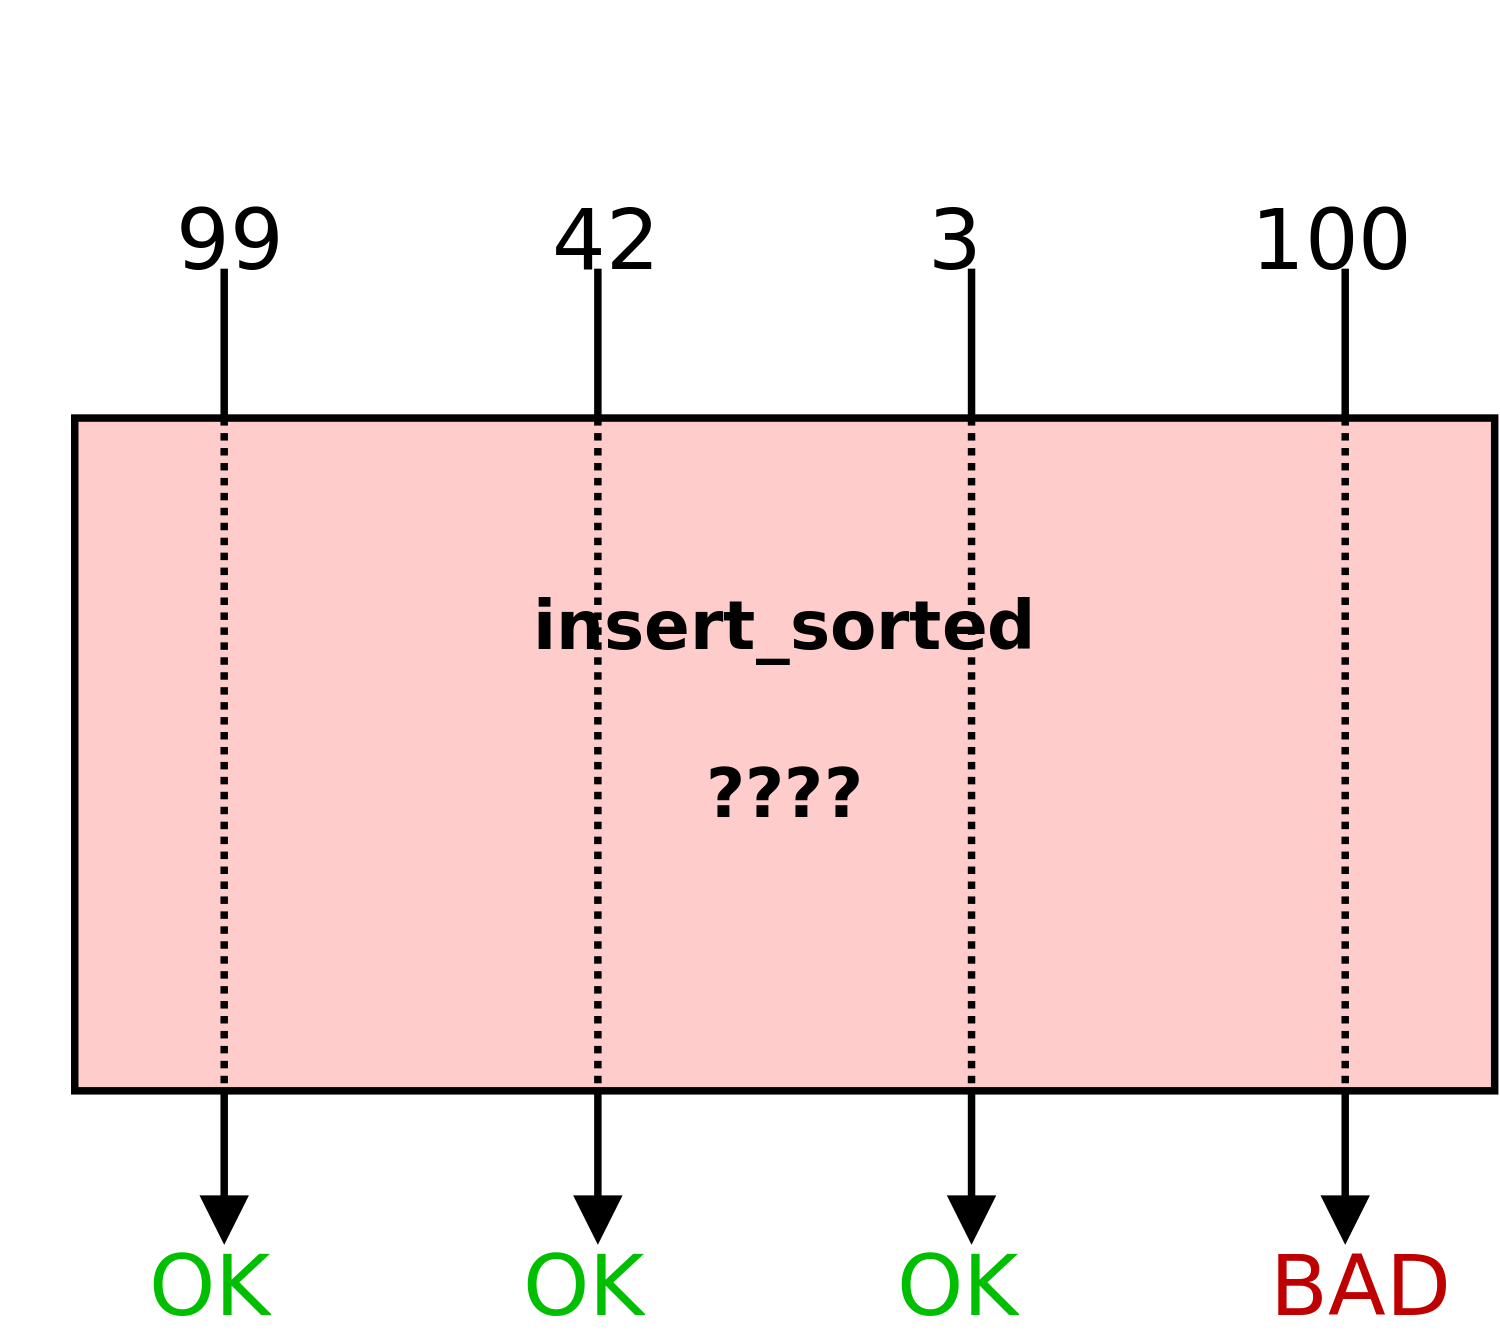
\includegraphics[width=0.65\textwidth]{space0.png}
	\end{center}
\end{frame}

\begin{frame}{Minimizing the Test Case}
	Which parts of your code are right?
	\begin{itemize}
		\item Write {\bf small tests that pass}
	\end{itemize}
	\linegap

	Which parts of your code are wrong?
	\begin{itemize}
		\item {\bf Minimize the failing test}
		\begin{itemize}
			\item Make it as small as possible, such that it still fails
		\end{itemize}
	\end{itemize}
	\pause
	\linegap

	\texttt{~~~~input~=~\hilight{brickred}{[99]};~~~~~\hilight{darkcyan}{//~OK}} \\
	\texttt{~~~~input~=~\hilight{brickred}{[100,99]};~\hilight{darkcyan}{//~OK}} \\
	\pause
	\texttt{~~~~input~=~\hilight{brickred}{[99,100]};~\hilight{darkcyan}{//~Fails}} \\
\end{frame}

\begin{frame}{Minimizing the Test Case}
	Old story:

	\begin{center}
	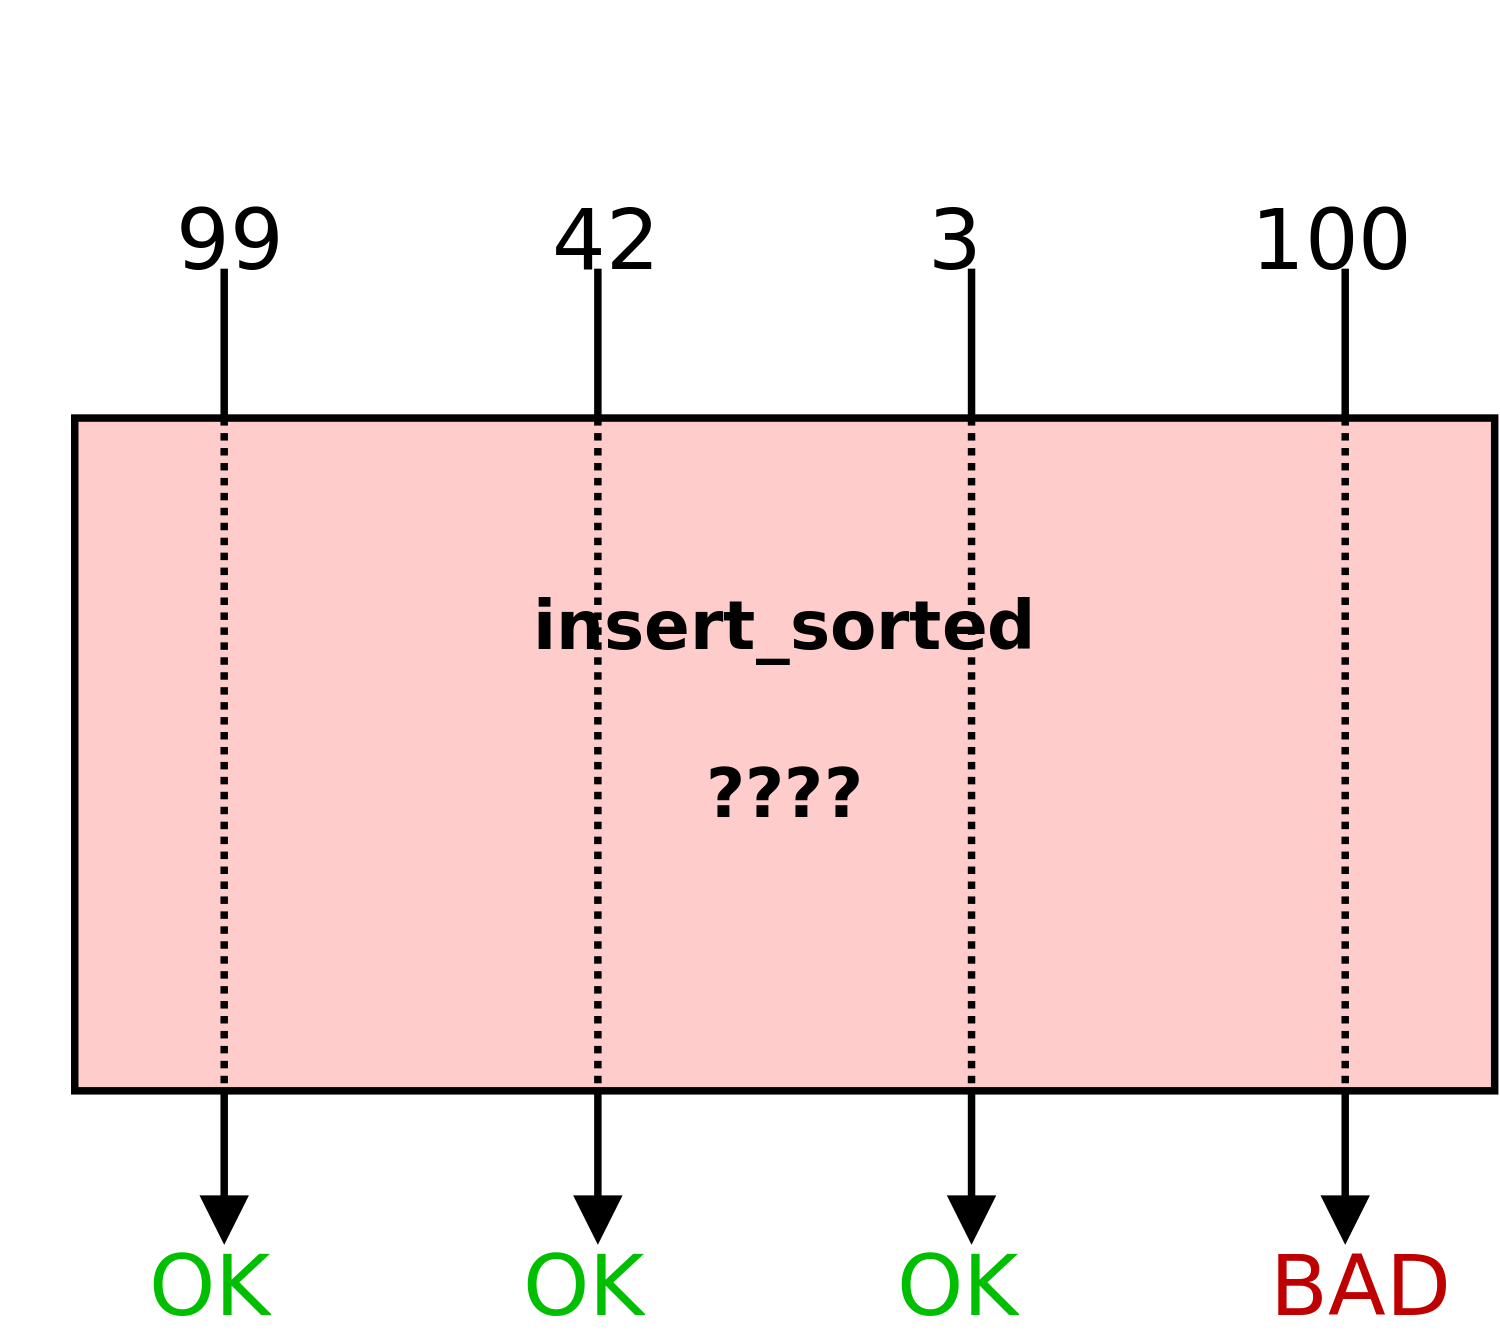
\includegraphics[width=0.65\textwidth]{space0.png}
	\end{center}
\end{frame}
\begin{frame}{Minimizing the Test Case}
	New story:

	\begin{center}
	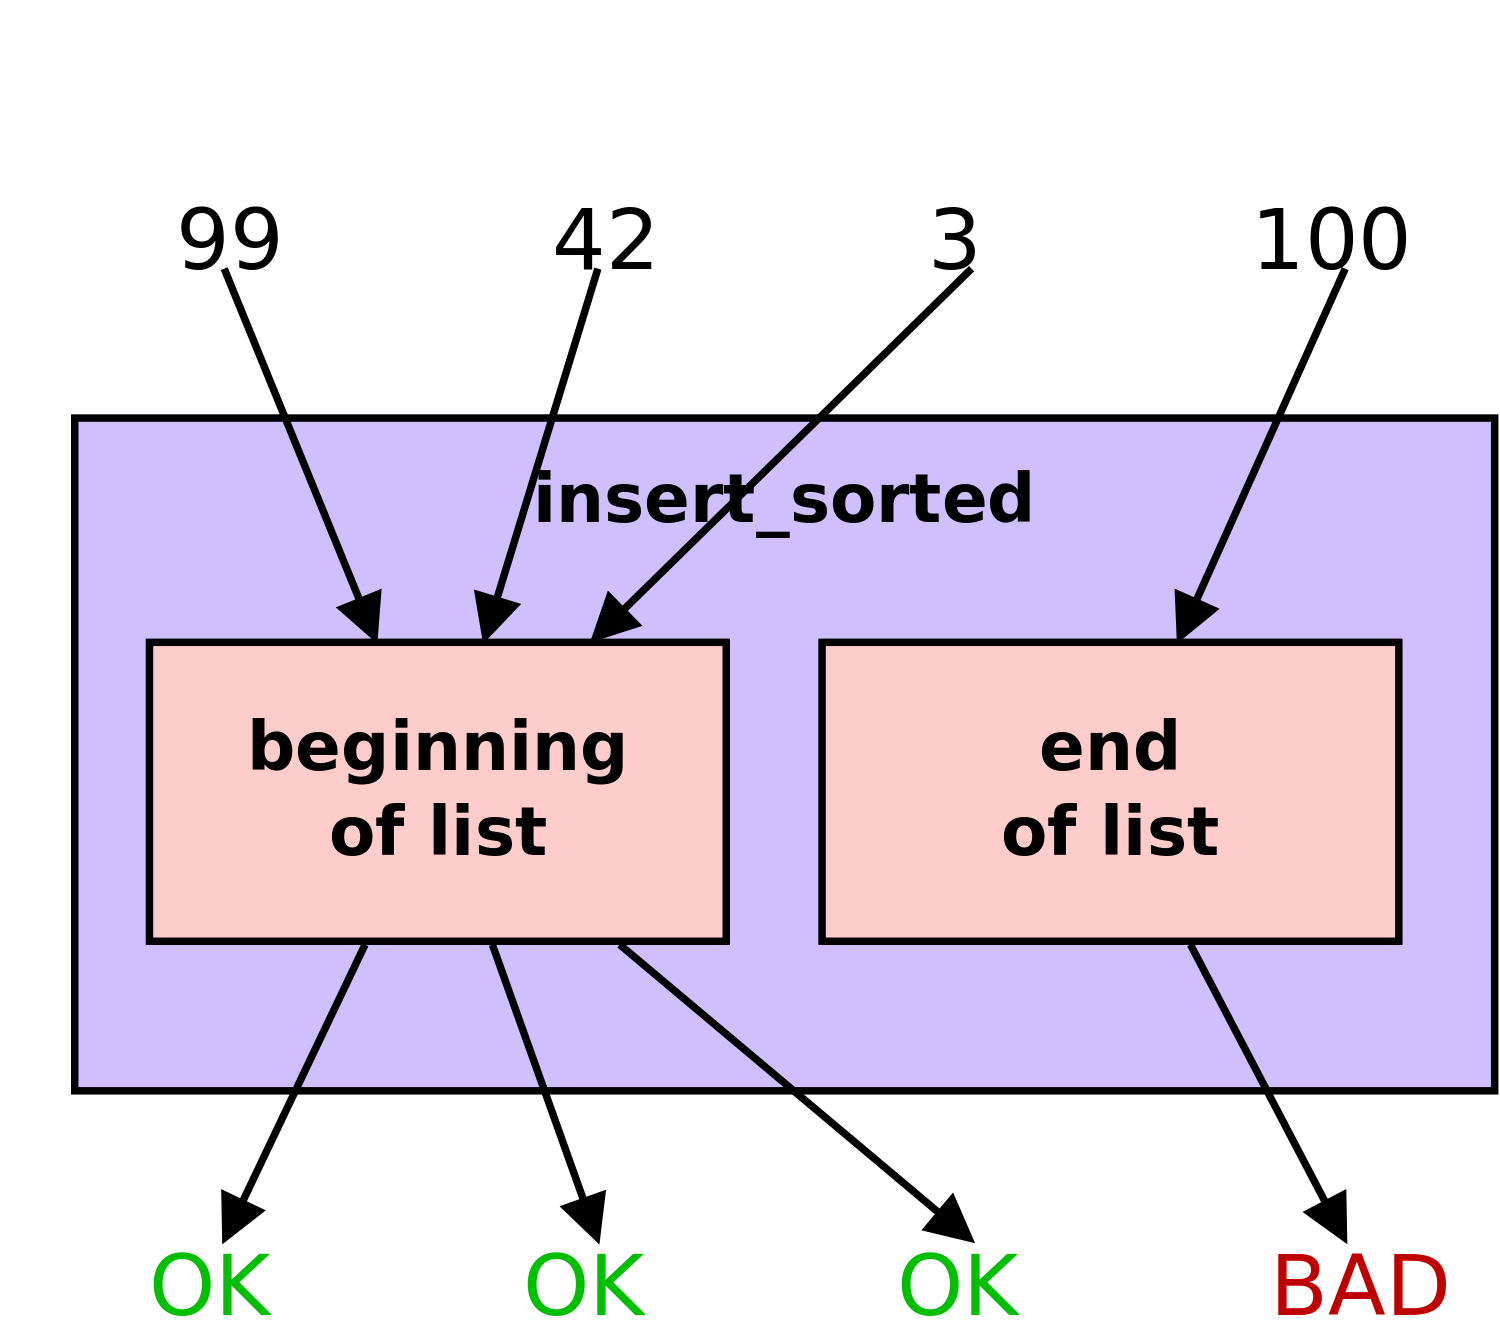
\includegraphics[width=0.65\textwidth]{space1.png}
	\end{center}
\end{frame}

%%%%%%%%%%%%%%%%%%%%%%%%%%%%%%%%%%%%%%%%%%%%%%%%%%%%%%%%%%%%%%%%%%%%%%%%%%%%%%%%
\section{Assorted Tips}
%%%%%%%%%%%%%%%%%%%%%%%%%%%%%%%%%%%%%%%%%%%%%%%%%%%%%%%%%%%%%%%%%%%%%%%%%%%%%%%%

\breakslide{Assorted Tips \\ {\normalsize (Useful stuff that isn't specifically about ``space'' or ``time'')}}

\begin{frame}{Rubber Duck / Cardboard Dog Debugging}
	\begin{columns}[l]
	\column{0.75\textwidth}
	Hacker folklore says: describe your problem to a duck!
	\begin{itemize}
		\item ``What could I possibly get out of talking to an inanimate object?''
	\end{itemize}
	\linegap

	\onslide<2->{
	Hearing yourself speak makes you {\bf question your assumptions}.
	\begin{itemize}
		\item ``The bug can't be in X.''
		\item ``Why not? Are you sure X works?''
	\end{itemize}
	\linegap

	Helps figure out what part of the story to start searching at
	}
	\column{0.25\textwidth}
	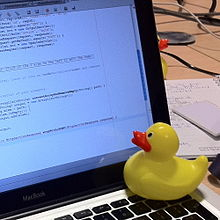
\includegraphics[width=\textwidth]{rubberduck.jpg}
	\end{columns}
\end{frame}
\begin{frame}{Rubber Duck / Cardboard Dog Debugging}
	\begin{columns}[l]
	\column{0.75\textwidth}
	{\em Question assumptions} also means {\em question explanations}.
	\begin{itemize}
		\item You: ``I think X is wrong''
		\item Duck: ``How can you be sure?''
	\end{itemize}
	\onslide<2->{
	\linegap
	The {\bf Hypothesis/Test} workflow
	\begin{itemize}
		\item Guess what the root cause is
		\item Write a small test that fails {\em iff} that's right.
		\onslide<3->{
		\begin{itemize}
			\item Not ``change code blindly, see if that fixes it''
			\item Until you know what's wrong, write {\em tests}
		\end{itemize}
		}
	\end{itemize}
	}
	\column{0.25\textwidth}
	\vspace{0.035in}
	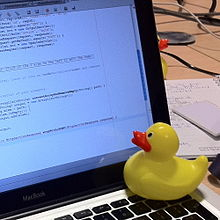
\includegraphics[width=\textwidth]{rubberduck.jpg}
	\end{columns}
\end{frame}

\begin{frame}{Draw Pictures}
	Draw what you think should happen

	Label relevant variables and their values
	\linegap

	\begin{center}
		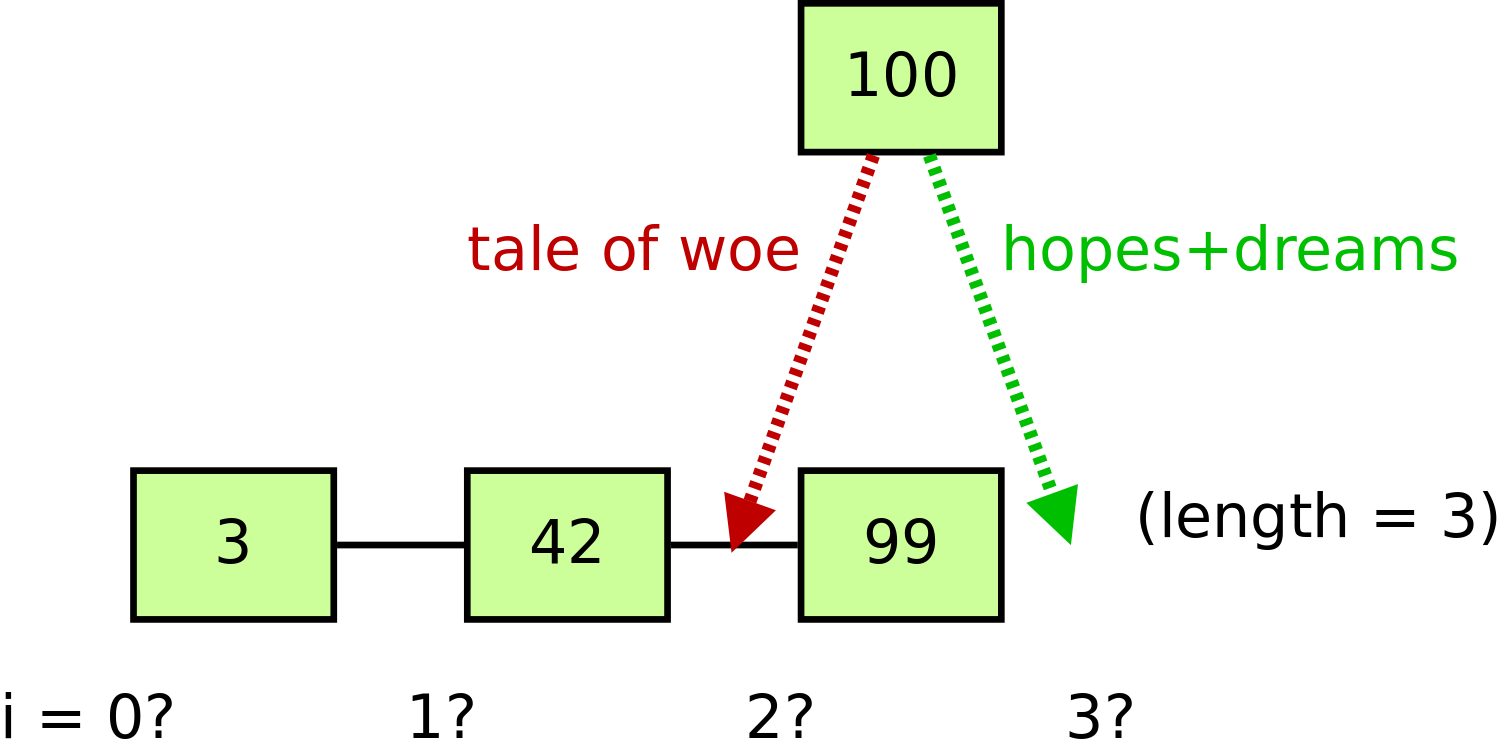
\includegraphics[width=0.8\textwidth]{draw-a-picture.png}
	\end{center}
\end{frame}

\begin{frame}{Binary Search}
	Print statements and unit tests create {\em bounds} on when the problem happened
	\begin{itemize}
		\item Iteratively making bounds smaller helps you hone in on the bug.
		\begin{itemize}
			\item Add more print statements
			\item Write unit tests to test many (small!) parts of the code
		\end{itemize}
		\item Hey wait, this sounds like a certain search algorithm...
	\end{itemize}
	\pause
	Binary search: ``$O(\mathsf{log}(n))$'' is not just talking about code!
	\linegap
	\pause

	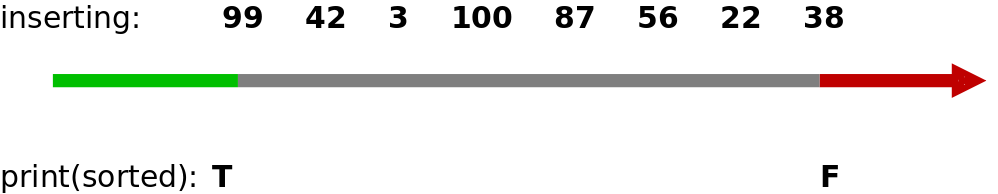
\includegraphics[width=\textwidth]{binary1.png}
\end{frame}
\begin{frame}{Binary Search}
	Print statements and unit tests create {\em bounds} on when the problem happened
	\begin{itemize}
		\item Iteratively making bounds smaller helps you hone in on the bug.
		\begin{itemize}
			\item Add more print statements
			\item Write unit tests to test many (small!) parts of the code
		\end{itemize}
		\item Hey wait, this sounds like a certain search algorithm...
	\end{itemize}
	Binary search: ``$O(\mathsf{log}(n))$'' is not just talking about code!
	\linegap

	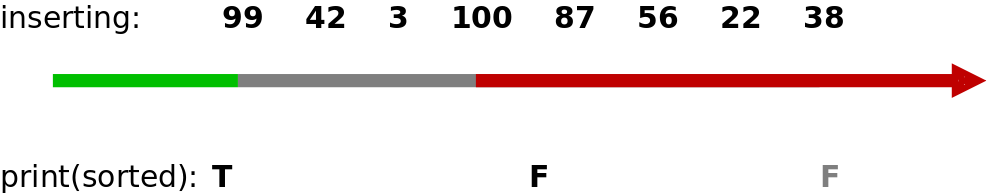
\includegraphics[width=\textwidth]{binary2.png}
\end{frame}
\begin{frame}{Binary Search}
	Print statements and unit tests create {\em bounds} on when the problem happened
	\begin{itemize}
		\item Iteratively making bounds smaller helps you hone in on the bug.
		\begin{itemize}
			\item Add more print statements
			\item Write unit tests to test many (small!) parts of the code
		\end{itemize}
		\item Hey wait, this sounds like a certain search algorithm...
	\end{itemize}
	Binary search: ``$O(\mathsf{log}(n))$'' is not just talking about code!
	\linegap

	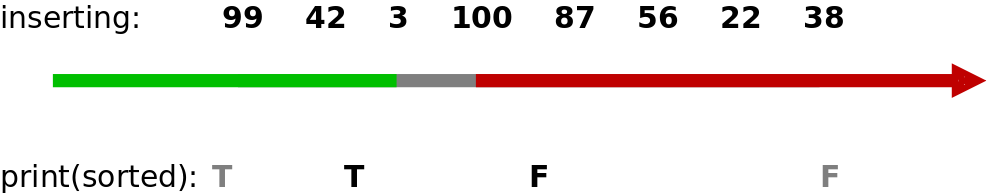
\includegraphics[width=\textwidth]{binary3.png}
\end{frame}
\begin{frame}{Binary Search}
	Print statements and unit tests create {\em bounds} on when the problem happened
	\begin{itemize}
		\item Iteratively making bounds smaller helps you hone in on the bug.
		\begin{itemize}
			\item Add more print statements
			\item Write unit tests to test many (small!) parts of the code
		\end{itemize}
		\item Hey wait, this sounds like a certain search algorithm...
	\end{itemize}
	Binary search: ``$O(\mathsf{log}(n))$'' is not just talking about code!
	\linegap

	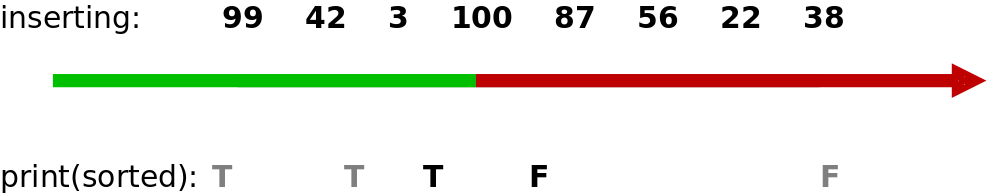
\includegraphics[width=\textwidth]{binary4.png}
\end{frame}
\begin{frame}{Binary Search}
	This also applies to ``space'', not just to ''time''
	\begin{itemize}
		\item Sometimes the only thing that makes your code crash is a 1000-line test case
		\begin{itemize}
			\item Binary search on ``which parts of the test need to be there''
		\end{itemize}
	\end{itemize}
	\pause
	\linegap
	Still don't believe me? \texttt{git bisect}
	\begin{itemize}
		\item Helps find which {\em git revision} introduced a bug
		\item Start with one ``known good'' revision, one ``known bad'' one
		\item \texttt{bisect} binary-searches on revisions in-between, asking you at each if it's good or bad.
	\end{itemize}
\end{frame}

\begin{frame}{One Last Aside: Repeatability}
	All the tests and bugs here have been {\em deterministic}.
	\begin{itemize}
		\item If you see the failure once, you can keep making it happen until it's fixed.
	\end{itemize}
	\pause
	\linegap

	In the ``real world'', and in 400-level classes, failures are not so easy to reproduce.
	\begin{itemize}
		\item Consider: \texttt{input = [rand(), rand(), rand(), rand()]}
		\item Might have failed last week, but never since
	\end{itemize}
	\pause
	\linegap
	Make sure your test cases are {\bf repeatable}
	\begin{itemize}
		\item Getting help (from a TA, from a company) easier when you say ``Here is a failing test'' than ''I once saw a test fail''!
		\item Nonrepeatable tests are often complex
		\begin{itemize}
			\item Use the rest of these techniques to produce a relevant, minimal failing test case.
		\end{itemize}
	\end{itemize}
\end{frame}

%%%%%%%%%%%%%%%%%%%%%%%%%%%%%%%%%%%%%%%%%%%%%%%%%%%%%%%%%%%%%%%%%%%%%%%%%%%%%%%%
\section{Conclusion}
%%%%%%%%%%%%%%%%%%%%%%%%%%%%%%%%%%%%%%%%%%%%%%%%%%%%%%%%%%%%%%%%%%%%%%%%%%%%%%%%

\breakslide{What's in this ``toolbox'', again? \\ {\normalsize (Conclusion)}}

\begin{frame}{The Toolbox}
	\begin{columns}[l]
	\column{0.05\textwidth}
	\column{0.5\textwidth}
	\textbf{``Tell Me a Story''}
	\begin{itemize}
		\item Get more detail
		\item Rinse \& repeat
		\pause
		\item {\bf Tell a Story of Time}
		\begin{itemize}
			\item Print debugging
			\item Asserts
		\end{itemize}
		\pause
		\item {\bf Tell a Story of Space}
		\begin{itemize}
			\item Minimize the failing test case
			\item Make small tests that work
		\end{itemize}
		\pause
		\item Draw pictures, collect data, question assumptions, binary search
	\end{itemize}
	\column{0.45\textwidth}
	\pause
	\begin{center}
		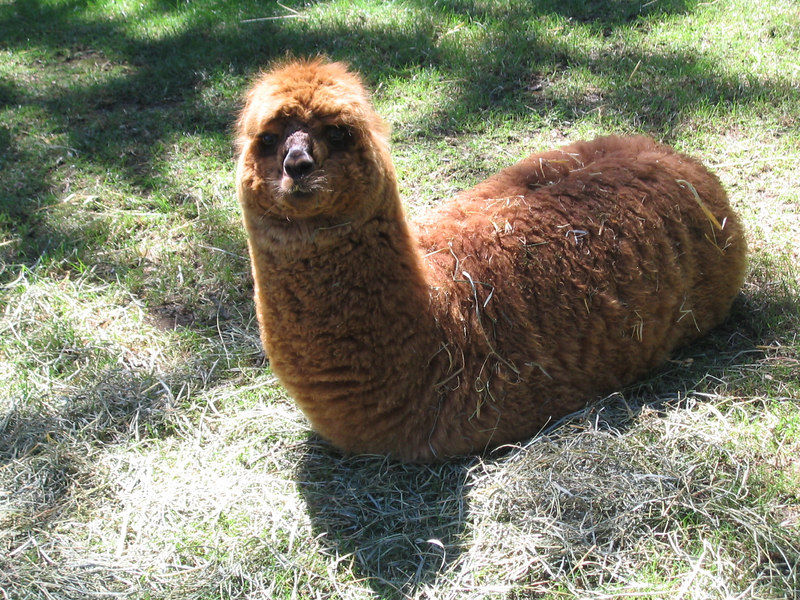
\includegraphics[width=0.9\textwidth]{vip1066720.jpg}
	\end{center}
	\end{columns}
\end{frame}

\end{document}
%%%%%%%%%%%%%%%%%%%%%%%%%%%%%%%%%%%%%%%%%%%%%%%%%%%%%%%%%%%%%%%%%%%%%%%%%%%%%%%%
% vim: foldmethod=indent
